\documentclass[dutch]{beamer}
%\documentclass[handout]{beamer}

%\usecolortheme{dove} %voor bij handout zodat er geen kleur meer inzit

\usepackage[dutch]{babel}
\usepackage{beamerthemesplit}
\usepackage{amsmath,latexsym,amssymb,graphicx,cancel}
\usepackage[latin1]{inputenc}
\usepackage{color}
\swapnumbers\newtheorem{stelling}{Stelling}[section]
\newtheorem{hulpstelling}[stelling]{Hulpstelling}
\newtheorem{gevolg}[stelling]{Gevolg}
\newtheorem{gevolgen}[stelling]{Gevolgen}
\newtheorem{voorbeeld}[stelling]{Voorbeeld}
\newtheorem{voorbeelden}[stelling]{Voorbeelden}
\newtheorem{belangrijkvoorbeeld}[stelling]{Belangrijk voorbeeld}
\newtheorem{belangrijkgevolg}[stelling]{Belangrijk gevolg}
\newtheorem{belangrijkegevolgen}[stelling]{Belangrijke gevolgen}
\newtheorem{opmerking}[stelling]{Opmerking}
\newtheorem{opmerkingen}[stelling]{Opmerkingen}
\newtheorem{definitie}[stelling]{Definitie}
\newtheorem{toepassing}[stelling]{Toepassing}
\newtheorem{oefeningen}[stelling]{Oefeningen}
\newtheorem{definities}[stelling]{Definities}
\newtheorem{oefening}[stelling]{Oefening}
\newtheorem{notatie}[stelling]{Notatie}
\def\bb{\begin{proof}[Bewijs]}
\def\eb{\end{proof}}
\def\bs{\begin{stelling}}
\def\es{\end{stelling}}
\def\bhs{\begin{hulpstelling}}
\def\ehs{\end{hulpstelling}}
\def\bg{\begin{gevolg}}
\def\eg{\end{gevolg}}
\def\bgn{\begin{gevolgen}\hfill\begin{enumerate}}
\def\egn{\end{enumerate}\end{gevolgen}}
\def\bv{\begin{voorbeeld}\rm}
\def\ev{\end{voorbeeld}}
\def\bbv{\begin{belangrijkvoorbeeld}\rm}
\def\ebv{\end{belangrijkvoorbeeld}}
\def\bbg{\begin{belangrijkgevolg}\rm}
\def\ebg{\end{belangrijkgevolg}}
\def\bbgn{\begin{belangrijkegevolgen}\rm}
\def\ebgn{\end{belangrijkegevolgen}}
\def\bt{\begin{toepassing}}
\def\et{\end{toepassing}}
\def\bn{\begin{notatie}\rm}
\def\en{\end{notatie}}
\def\bvn{\begin{voorbeelden}\hfill\begin{enumerate}\rm}
\def\evn{\end{enumerate}\end{voorbeelden}}
\def\bo{\begin{opmerking}\rm}
\def\eo{\end{opmerking}}
\def\bon{\begin{opmerkingen}\hfill\begin{enumerate}\rm }
\def\eon{\end{enumerate}\end{opmerkingen}}
\def\bd{\begin{definitie}\rm}
\def\ed{\end{definitie}}
\def\bds{\begin{definities}\rm}
\def\eds{\end{definities}}
\def\ds{\displaystyle}
\newcommand{\R}{\mathbb{R}}
\newcommand{\Q}{\mathbb{Q}}
\newcommand{\Z}{\mathbb{Z}}
\newcommand{\N}{\mathbb{N}}
\newcommand{\A}{\mathcal{A}}
\newcommand{\B}{\mathcal{B}}
\renewcommand{\L}{\mathcal{L}}
\newcommand{\ubar}[1]{\text{{\itshape\b #1}\,}}
\DeclareMathOperator*{\ulim}{\underline{\lim}}
\DeclareMathOperator*{\blim}{\overline{\lim}}
\usepackage{color}

%\setbeamercovered{transparent}


\def\bfi{\boldsymbol{\varphi}}
\def\bp{\boldsymbol{\psi}}
\def\vf{\mathbf f}
\def\bc{\mathbf c}

\def\kg{\leqslant}
\def\gg{\geqslant}


\def\eps{\varepsilon} 
\def\leeg{\varnothing}
\def\N{\mathbb  N}
\def\Z{\mathbb  Z}
\def\Q{\mathbb  Q}
\def\R{\mathbb  R}
\def\C{\mathbb  C}

\def\bl{\varlimsup\limits}
\def\ongelijkkleiner#1{\overset{\,<}{#1}}
\def\ongelijkgroter#1{\overset{\,>}{#1}}
\def\inw#1{\overset{\,\,\circ}{#1}}
\def\bl{\varlimsup}
\def\ol{\varliminf}

\def\arb{D^\circ\!}
\def\aro{D_\circ}
\def\alb{{}^\circ\!D}
\def\alo{{}_\circ D}
\def\aprb{A^\circ\!}
\def\apro{A_\circ}
\def\aplb{{}^\circ\!A}
\def\aplo{{}_\circ A}
\def\bprb{B^\circ\!}
\def\bpro{B_\circ}
\def\bplb{{}^\circ\!B}
\def\bplo{{}_\circ B}
\def\drb{d^\circ\!}
\def\dro{d_\circ}
\def\dlb{{}^\circ\!d}
\def\dlo{{}_\circ d}


\DeclareMathOperator{\diam}{diam}
\DeclareMathOperator{\opp}{opp}
\DeclareMathOperator{\rot}{rot}
\DeclareMathOperator{\volu}{vol}
\DeclareMathOperator{\diver}{div}


%\usetheme{Copenhagen}
%\usecolortheme{dolphins}
%rgb ---> 0.3,0.5,0.7 mooi blauw
\usetheme{antibes}
%\definecolor{mycolor}{RGB}{48,96,102}
%\definecolor{mycolor2}{RGB}{63,125,133}
%\setbeamercolor*{palette primary}{use=structure,fg=white,bg=mycolor}
\setbeamertemplate{navigation symbols}{}

%\newenvironment{colorblock}[1]
%{\setbeamercolor{item}{fg=mycolor}\begin{beamerboxesrounded}}
%{\end{beamerboxesrounded}}


\title[Bolstapelprobleem van Kepler]{Quiz Bolstapelprobleem}
%\author[]{Lien Lambert \\ Pieter Pareit \\ Jordy Vanpoucke}
\date{}


\begin{document}
\newcommand{\rechtsboven}[1]{D^\circ\! f(#1)}
\newcommand{\rechtsonder}[1]{D_\circ f(#1)}
\newcommand{\linksboven}[1]{{}^\circ\! Df(#1)}
\newcommand{\linksonder}[1]{{}_\circ Df(#1)}
\newcommand{\rechtsbovenmin}[1]{D^\circ\!(f(-#1))}
\newcommand{\rechtsondermin}[1]{D_\circ (f(-#1))}
\newcommand{\linksbovenmin}[1]{{}^\circ\!D(f(-#1))}
\newcommand{\linksondermin}[1]{{}_\circ D(f(-#1))}
\newcommand{\minrechtsboven}[1]{D^\circ\! (-f(#1))}
\newcommand{\minrechtsonder}[1]{D_\circ (-f(#1))}
\newcommand{\minlinksboven}[1]{{}^\circ\!D(-f(#1))}
\newcommand{\minlinksonder}[1]{{}_\circ D(-f(#1))}
\frame{
%\begin{figure}[t]
%	\flushleft
%		\includegraphics[scale=0.1]{logo.jpg}
%\end{figure}
\titlepage

\begin{figure}[h]
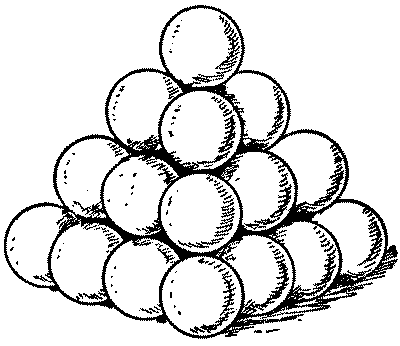
\includegraphics[width=4cm]{cannonballs}
\end{figure}
}
\section{Ontstaan}
\subsection{Vraag 1}
\begin{frame}

\begin{block}
{Wie was de wetenschappelijk adviseur van Sir Walter Raleigh?}

\begin{itemize}
	\item[A] Thomas Harriot
	\item[B] Johannes Kepler
	\item[C] Hij had geen wetenschappelijk adviseur
\end{itemize}
\end{block}

\begin{figure}
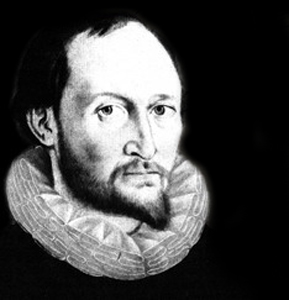
\includegraphics[height=3cm]{harriot}
\end{figure}


\end{frame}

\begin{frame}

\begin{block}
{Wie was de wetenschappelijk adviseur van Sir Walter Raleigh?}

\begin{itemize}
	\item[\textbf{A}] \textbf{Thomas Harriot}
	\item[B] Johannes Kepler
	\item[C] Hij had geen wetenschappelijk adviseur
\end{itemize}
\end{block}

\begin{figure}
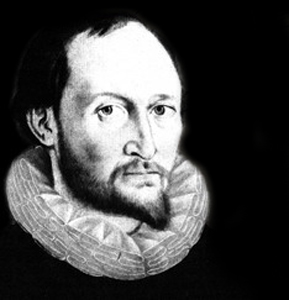
\includegraphics[height=3cm]{harriot}
\end{figure}


\end{frame}

\subsection{Vraag 2}

\begin{frame}

\begin{block}
{Wat is de nationaliteit van Johannes Kepler?}

\begin{itemize}
	\item[A] Duitser
	\item[B] Oostenrijker
	\item[C] Engelsman
	\end{itemize}
\end{block}
\begin{figure}[h]
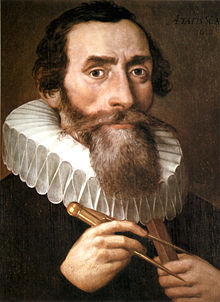
\includegraphics[heigth=5cm]{kepler}

\end{figure}

\end{frame}


\begin{frame}

\begin{block}
{Wat is de nationaliteit van Johannes Kepler?}

\begin{itemize}
	\item[\textbf{A}] \textbf{Duitser}
	\item[B] Oostenrijker
	\item[C] Engelsman
	\end{itemize}
\end{block}
\begin{figure}[h]
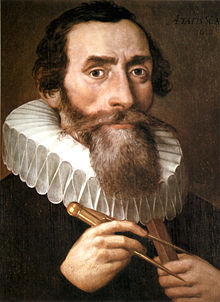
\includegraphics[heigth=5cm]{kepler}

\end{figure}

\end{frame}


\subsection{Vraag 3 }
\begin{frame}

\begin{block}
{Welke term betekent niet 'het maximum aantal niet-overlappende eenheidssferen dat aan een gegeven eenheidssfeer raakt'?}

\begin{itemize}
	\item[A] Newton number
	\item[B] Kissing number
	\item[C] Contact number
	\item[D] Kepler number
	\end{itemize}
\end{block}

\begin{figure}[h]
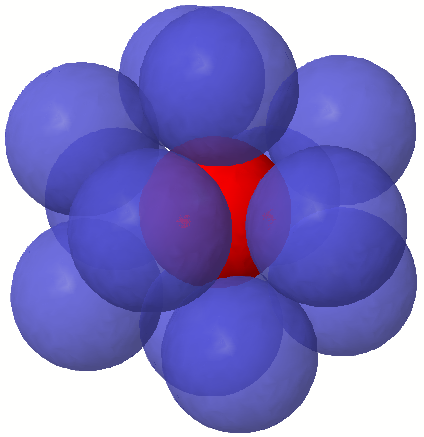
\includegraphics[width=3cm]{kissing}
\end{figure}
%D

\end{frame}

\begin{frame}

\begin{block}
{Welke term betekent niet 'het maximum aantal niet-overlappende eenheidssferen dat aan een gegeven eenheidssfeer raakt'?}

\begin{itemize}
	\item[A] Newton number
	\item[B] Kissing number
	\item[C] Contact number
	\item[\textbf{D}] \textbf{Keper number}
	\end{itemize}
\end{block}

\begin{figure}[h]
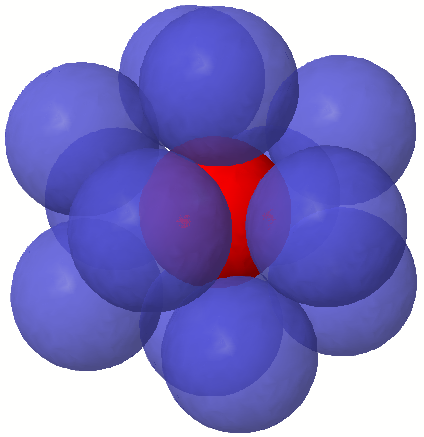
\includegraphics[width=3cm]{kissing}
\end{figure}
%D

\end{frame}


\section{Evolutie}
\subsection{Vraag 4}

\begin{frame}

\begin{block}{Welke Duitse Wiskundige bewees dat de \textquoteleft face-centered cubic packing' de dichtste pakkingsmethode is volgens een rooster?}
\begin{itemize}
	\item[A] Kepler
	\item[B] Gauss
	\item[C] Hilbert 
\end{itemize}
\end{block}

\begin{figure}[h]
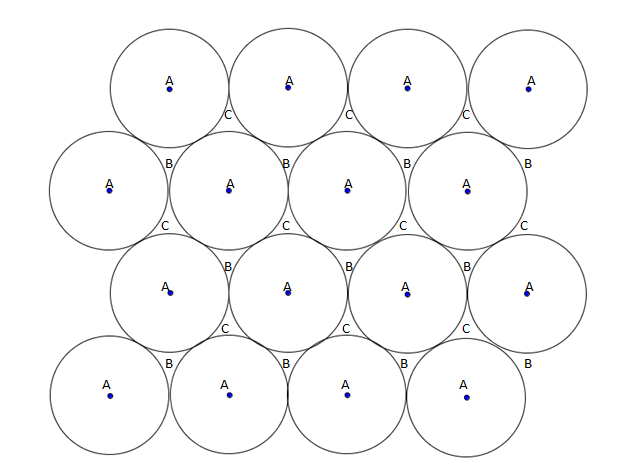
\includegraphics[height=3cm]{fcc}
\end{figure}
\end{frame}

\begin{frame}

\begin{block}{Welke Duitse Wiskundige bewees dat de \textquoteleft face-centered cubic packing' de dichtste pakkingsmethode is volgens een rooster?}
\begin{itemize}
	\item[A] Kepler
	\item[\textbf{B}] \textbf{Gauss}
	\item[C] Hilbert 
\end{itemize}
\end{block}

\begin{figure}[h]
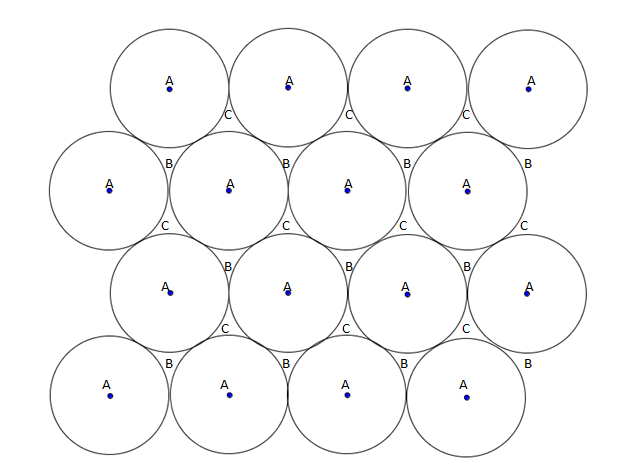
\includegraphics[height=3cm]{fcc}
\end{figure}
\end{frame}


\subsection{Vraag 5}

\begin{frame}
\begin{block}
{Welke Scandinavische wiskundige ontwikkelde een theorie over het tweedimensionale equivalent voor 'het probleem van Kepler' waarin men zicht naar de dichtste pakkingsmethode voor cirkels in het vlak?}

\begin{itemize}
	\item[A] Axel Thue
	\item[B] L�szlo Feje T�th
	\item[C] Wu-Yi Hsiang
	\end{itemize}
\end{block}

\begin{figure}[h]
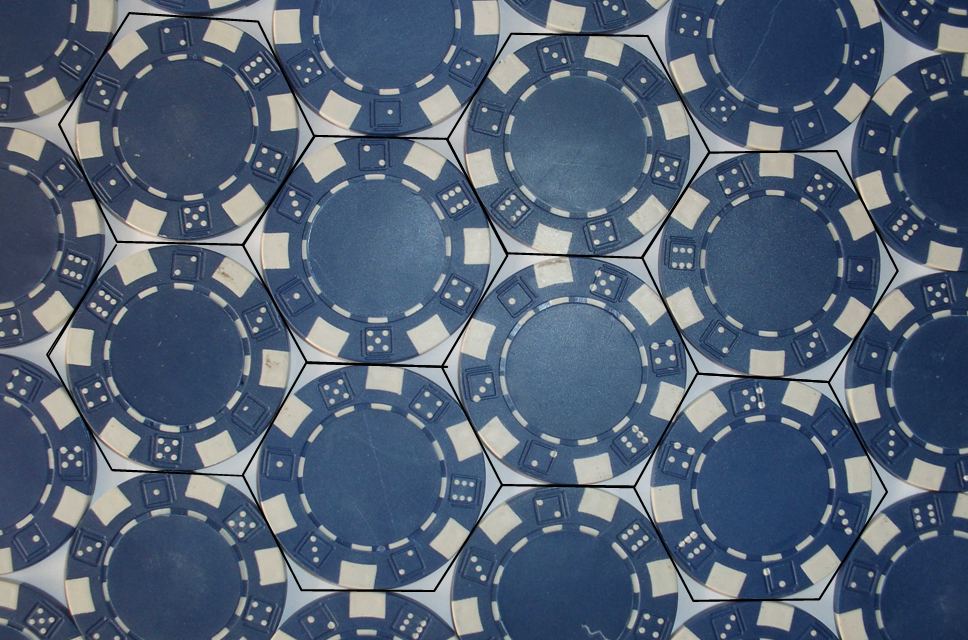
\includegraphics[width=3cm]{voronoi_hex}
\end{figure}

\end{frame}

\begin{frame}
\begin{block}
{Welke Scandinavische wiskundige ontwikkelde een theorie over het tweedimensionale equivalent voor 'het probleem van Kepler' waarin men zicht naar de dichtste pakkingsmethode voor cirkels in het vlak?}

\begin{itemize}
	\item[\textbf{A}] \textbf{Axel Thue}
	\item[B] L�szlo Feje T�th
	\item[C] Wu-Yi Hsiang
	\end{itemize}
\end{block}

\begin{figure}[h]
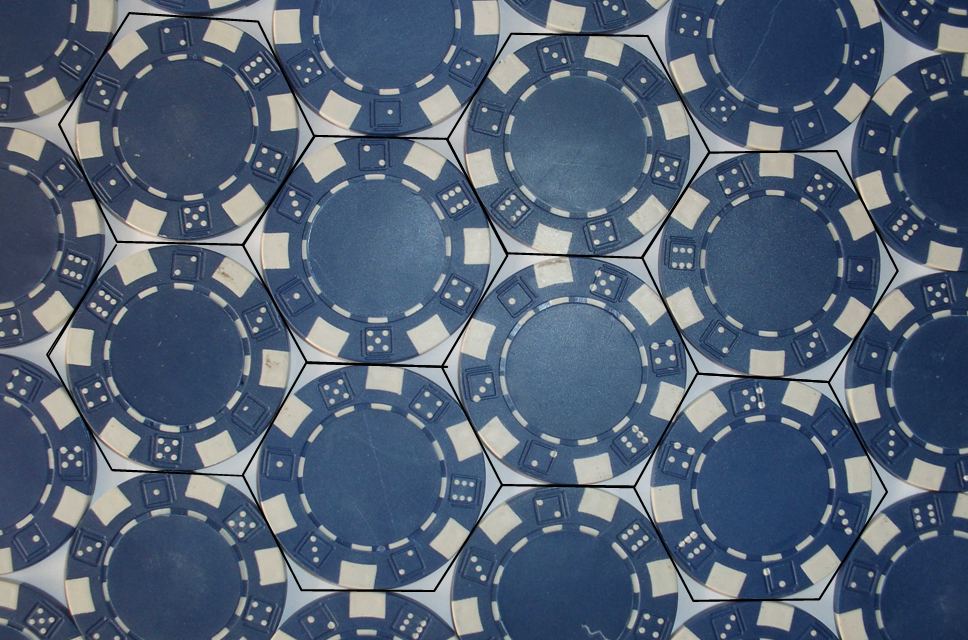
\includegraphics[width=3cm]{voronoi_hex}
\end{figure}

\end{frame}

\subsection{Vraag 6}

\begin{frame}
\begin{block}
{Kepler vermoedde dat de dichtheid van de dichtste bolstapeling $\frac{\pi}{\sqrt{18}}$ is. Wat is deze effici�ntie als percentage?}

\begin{itemize}
	\item[A] 74,0480 \%
	\item[B] 77,964 \%
	\item[C] 77,844 \%
	\item[D] 77,3055 \%
	\end{itemize}
\end{block}


\end{frame}


\begin{frame}
\begin{block}
{Kepler vermoedde dat de dichtheid van de dichtste bolstapeling $\frac{\pi}{\sqrt{18}}$ is. Wat is deze effici�ntie als percentage?}

\begin{itemize}
	\item[\textbf{A}] \textbf{74,0480 \%}
	\item[B] 77,964 \%
	\item[C] 77,844 \%
	\item[D] 77,3055 \%
	\end{itemize}
\end{block}

\end{frame}
\section{Bewijs}
\subsection{Vraag 7}

\begin{frame}
\begin{block}
{Voor hoeveel stapelingen moest Thomas Hales uiteindelijk het probleem van Kepler aantonen?}

\begin{itemize}
	\item[A] 5
	\item[B] 50
	\item[C] 500
	\item[D] 5000
	\end{itemize}
\end{block}

\begin{figure}[h]
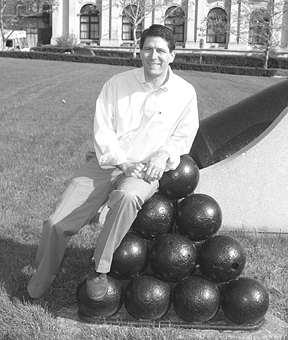
\includegraphics[width=3cm]{hales}
\end{figure}

\end{frame}


\begin{frame}
\begin{block}
{Voor hoeveel stapelingen moest Thomas Hales uiteindelijk het probleem van Kepler aantonen?}

\begin{itemize}
	\item[A] 5
	\item[B] 50
	\item[C] 500
	\item[\textbf{D}] \textbf{5000}
	\end{itemize}
\end{block}

\begin{figure}[h]
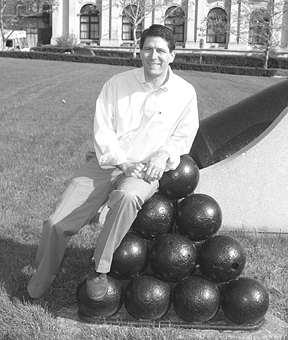
\includegraphics[width=3cm]{hales}
\end{figure}

\end{frame}

\subsection{Vraag 8}

\begin{frame}
\begin{block}
{Waarom bleken er voor sommigen achteraf nog twijfels over het bewijs van Hales ?}

\begin{itemize}
	\item[A] Eigenlijk was het zijn assistent Samuel Ferguson die het bewijs had geleverd.
	\item[B] Het bewijs is zo lang dat het niet gecontroleerd kan worden.
	\item[C] Hales bewees de stelling met de computer.
	\end{itemize}
\end{block}

\begin{figure}[h]
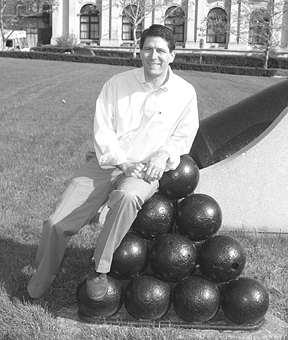
\includegraphics[width=3cm]{hales}
\end{figure}

\end{frame}


\begin{frame}
\begin{block}
{Waarom bleken er voor sommigen achteraf nog twijfels over het bewijs van Hales ?}

\begin{itemize}
	\item[A] Eigenlijk was het zijn assistent Samuel Ferguson die het bewijs had geleverd.
	\item[B] Het bewijs is zo lang dat het niet gecontroleerd kan worden.
	\item[\textbf{C}] \textbf{Hales bewees de stelling met de computer.}
	\end{itemize}
\end{block}

\begin{figure}[h]
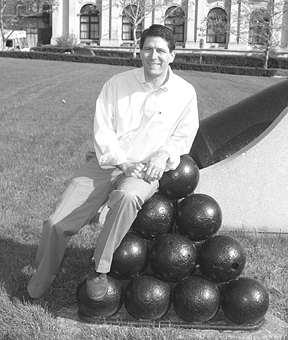
\includegraphics[width=3cm]{hales}
\end{figure}

\end{frame}


\end{document}